% arara: pdflatex
% arara: clean : {extensions:[aux,bbl,bcf,blg,glg,glo,gls,idx,ilg,ind,ist,lof,lol,lot,nlo,nls,out,ptc,toc,run.xml]}
\documentclass[12pt]{article} % use the article class

%%% The following looks horrible, but essentially sets up biblatex for producing
%%% bibliographies that look nice (you likely will not even need this)
% \usepackage[style=authoryear-comp, maxcitenames=2, isbn=false, url=false,
%     giveninits=true, doi=false, eprint=false, dashed=false, date=year,
%     related=false, mergedate=true]{biblatex}
% \renewbibmacro{in:}{%
%     \ifboolexpr{%
%         test {\ifentrytype{article}}%
%         or
%         test {\ifentrytype{inproceedings}}%
%     }{}{\printtext{\bibstring{in}\intitlepunct}}%
% }
% \renewbibmacro*{cite:labelyear+extrayear}{%
%     \ifentrytype{online}
%     {}
%     {\iffieldundef{labelyear}
%         {}
%         {\printtext[bibhyperref]{%
%                 \printfield{labelyear}
%                 \printfield{extrayear}}}}}

% \AtEveryBibitem{%
%     \clearfield{pagetotal}%
% }

% \DeclareFieldFormat[article,inbook,incollection,techreport,inproceedings,patent,thesis,unpublished]{title}{#1\isdot}
% \DeclareFieldFormat{pages}{#1}

\usepackage[plain]{algorithm} % algorithms package
\usepackage{algpseudocode} % pseudo-code package
\usepackage{amsbsy} % for producing bold maths symbols
\usepackage{amsfonts} % an extended set of fonts for maths
\usepackage{amssymb} % various maths symbols
\usepackage{amsthm} % for producing theorem-like environments
\usepackage{datetime2} % managing dates and times
\usepackage{delimseasy} % makes easy the manual sizing of brackets, square brackets, and curly brackets
\usepackage{enumitem} % customing list environments
\usepackage{extramarks} % extra marks
\usepackage{fancyhdr} % headers and footers
\usepackage{float} % makes dealing with floats (e.g. tables and figures) easier
\usepackage{framed} % for producing framed boxes
\usepackage{graphicx} % for including graphics in the document
\usepackage{hyperref} % automatically produce hyperlinks for cross-references
\usepackage{mathtools} % package for maths (fixes some deficiences of amsmath so is preferred)
\usepackage{microtype} % better font sizing (extremely helpful with long equations!)
\usepackage{newtx} % a fonts package
\usepackage{pdfpages} % for including pdf documents inside the compiled pdf
\usepackage{pgf} % produce pdf graphics using LaTeX
\usepackage{pgfplots} % create normal/logarithmic plots in two and three dimensions
\pgfplotsset{compat=1.18} % sorts out the compatability warning
\usepackage{physics} % useful for vector calculus and linear algebra symbols
\usepackage[theorems]{tcolorbox} % for producing coloured boxes
\tcbuselibrary{theorems} % theorems with tcolorbox
\usepackage{tikz-3dplot} % for producing 3d plots
\usepackage{tikz} % for drawing graphics in LaTeX
\usepackage{tkz-base} % drawing with a Cartesian coordinate system
\usepackage{tkz-euclide} % drawing in Euclidean geometry
\usepackage{xcolor} % a package for colours
\usepackage{minted}
\usepackage{relsize}
\usepackage[spanish]{babel}
\usepackage{caption}
\usepackage{subcaption}
\usepackage{placeins}
\usepackage{parskip}
\usepackage{pgfplotstable}

\usetikzlibrary{automata, positioning}

\DeclareMathAlphabet{\mathcal}{OMS}{cmsy}{m}{n}
 % imports the packages.tex file from the preamble directory
\renewcommand{\part}[1]{\textbf{\large Part \Alph{partCounter}}\stepcounter{partCounter}\\} % part macro
\newcommand{\solution}{\textbf{\large Solution}} % solution macro

% General writing
\newcommand{\bracket}[1]{\left(#1\right)} % for automatic resizing of brackets
\newcommand{\sbracket}[1]{\left[#1\right]} % for automatic resizing of square brackets
\newcommand{\mset}[1]{\left\{#1\right\}} % for automatic resizing of curly brackets
\newcommand{\defeq}{\coloneqq} % the "defined as" command
\newcommand{\ndash}{--\ } % for producing a dash
\newcommand{\mdash}{---\ } % for producing a longer dash
\newcommand{\by}{\times} % used for talking about m by n matrices
\newcommand{\eg}{e.g.\ } % for example
\newcommand{\ie}{i.e.\ } % i.e.
\newcommand{\RNum}[1]{\uppercase\expandafter{\romannumeral #1\relax}} % uppercase roman numerals
\renewcommand{\cite}{\textcite} % easier citing
\newcommand{\hide}[1]{} % useful for temporarily removing some code

\newcommand{\rednote}[1]{{\color{red} #1}} % for red text
\newcommand{\bluenote}[1]{{\color{blue} #1}} % for blue text
\newcommand{\greennote}[1]{{\color{green} #1}} % for green text

% Blackboard Maths Symbols
\newcommand{\N}{\mathbb{N}} % natural numbers
\newcommand{\Q}{\mathbb{Q}} % rational numbers
\newcommand{\Z}{\mathbb{Z}} % integers
\newcommand{\R}{\mathbb{R}} % real numbers
\newcommand{\C}{\mathbb{C}} % complex numbers
\newcommand{\E}{\mathbb{E}} % expectaion operators
\renewcommand{\P}{\mathbb{P}} % probability measures

% Calligraphic Maths Symbols
\newcommand{\F}{\mathcal{F}} % sigma-field

% Bold Maths Symbols
\newcommand{\1}{\mathbf{1}} % characteristic function

% Maths operations
\newcommand{\union}{\cup} % union
\newcommand{\intersect}{\cap} % intersection
\newcommand{\directsum}{\oplus} % direct sum
\newcommand{\Union}{\bigcup} % bigger union symbol
\newcommand{\Intersect}{\bigcap} % bigger intersection symbol
\newcommand{\Directsum}{\bigoplus} % bigger direct sum symbol
\newcommand{\tensor}{\otimes} % tensor
\newcommand{\Tensor}{\bigotimes} % bigger tensor symbol
\newcommand{\remove}{\setminus} % set difference
\renewcommand{\hom}[2]{\operatorname{Hom}\bracket{{#1}, {#2}}} % Hom sets

% Maths operations
\newcommand{\powerset}[1]{\mathcal{P}\bracket{#1}} % powerset
\renewcommand{\ip}[3]{\left \langle #1, #2 \right \rangle_{#3}} % inner product
\newcommand{\cardinality}[1]{\operatorname{Card}\bracket{#1}} % cardinality
\newcommand{\inv}[1]{#1^{-1}} % inverse
\newcommand{\adj}[1]{#1^{*}} % adjoint
\newcommand{\conj}[1]{\overline{#1}} % conjugate
\newcommand{\vspan}[1]{\operatorname{Span}\left\{#1\right\}} % vector space span
\renewcommand{\rank}[1]{\operatorname{Rank}\bracket{#1}} % rank of a linear transformation
\newcommand{\diag}[1]{\operatorname{Diag}\bracket{#1}} % diagonal elements of a square matrix
\renewcommand{\tr}[1]{\operatorname{Tr}\bracket{#1}} % trace
\newcommand{\kernel}[1]{\operatorname{Ker}\bracket{#1}} % kernel
\newcommand{\im}[1]{\operatorname{Im}\bracket{#1}} % image
\newcommand{\range}[1]{\operatorname{Ran}\bracket{#1}} % range
\newcommand{\col}[1]{\operatorname{Col}\bracket{#1}} % column space
\renewcommand{\exponential}[1]{\operatorname{exp}\bracket{#1}} % exponential function
\newcommand{\floor}[1]{\left\lfloor#1\right\rfloor} % macro for the floor function
\renewcommand{\ceil}[1]{\left\lceil#1\right\rceil} % macro for the ceiling function
\newcommand{\dx}{\,\mathrm{d}x} % differential of x
\newcommand{\dy}{\,\mathrm{d}y} % differential of y
\newcommand{\dt}{\,\mathrm{d}t} % differential of t


% optimisation objectives
\DeclareMathOperator*{\argmin}{argmin} % argument which minimises some criterion
\DeclareMathOperator*{\argmax}{argmax} % argument which maximises some criterion
\DeclareMathOperator*{\arginf}{arginf} % argument that gives the infimum of some criterion
\DeclareMathOperator*{\argsup}{argsup} % argument that gives the supremum of some criterion

% Statistical operations
\newcommand{\given}{\vert} % given (used in conditional probability)
\newcommand{\suchthat}{\;\middle|\;} % such that
\newcommand{\probspace}{\bracket{\Omega, \F, \P}} % a probability space
\newcommand{\borel}[1]{\B\bracket{#1}} % the Borel sigma-field
\newcommand{\prob}[1]{\P\bracket{#1}} % Probability
\newcommand{\cprob}[2]{\P\bracket{#1 \middle\given #2}} % Conditional probability
\newcommand{\expect}[1]{\E\bracket{#1}} % Expectation
\newcommand{\cexpect}[2]{\E\bracket{#1 \middle\given #2}} % Conditional expectation
\renewcommand{\var}[1]{\operatorname{Var}\bracket{#1}} % Variance
\newcommand{\cvar}[2]{\operatorname{Var}\bracket{#1 \middle\given #2}} % Conditional variance
\newcommand{\cov}[2]{\operatorname{Cov}\bracket{#1, #2}} % Covariance
\newcommand{\ccov}[3]{\operatorname{Cov}\bracket{#1, #2 \middle\given #3}} % Conditional covariance
\newcommand{\corr}[2]{\operatorname{Corr}\bracket{#1, #2}} % Correlation
\newcommand{\ccorr}[3]{\operatorname{Corr}\bracket{#1, #2 \middle\given #3}} % Conditional correlation

% Statistical symbols
\newcommand{\indep}{\perp\!\!\!\!\!\perp} % statistical independence
\newcommand{\sigfield}[1]{\sigma\bracket{#1}} % sigma-field
\newcommand{\evalue}[1]{\lambda_{#1}} % eigenvalue

\newcommand{\figuras}[2] {
    \begin{figure}[ht]
        \centering
        \begin{subfigure}{.5\textwidth}
            \centering
            \includegraphics[width=1\linewidth]{#1_aptitud_poblacion}
            \caption{Aptitud promedio de la población final}
            \label{fig:#1_1}
        \end{subfigure}%Misma fila
        \begin{subfigure}{.5\textwidth}
            \centering
            \includegraphics[width=1\linewidth]{#1_aptitud_individuo}
            \caption{Aptitud promedio del mejor individuo}
            \label{fig:#1_2}
        \end{subfigure}
        \begin{subfigure}{.5\textwidth}
            \centering
            \includegraphics[width=1\linewidth]{#1_iteraciones}
            \caption{Cantidad de iteraciones promedio}
            \label{fig:#1_3}
        \end{subfigure}%Misma fila
        \begin{subfigure}{.5\textwidth}
            \centering
            \includegraphics[width=1\linewidth]{#1_tiempo}
            \caption{Tiempo de ejecución promedio}
            \label{fig:#1_4}
        \end{subfigure}
        \caption{#2}
        \label{fig:#1}
    \end{figure}
    \FloatBarrier
} % imports the macros.tex file from the preamble directory
%%% DOCUMENT SETTINGS
\topmargin=-0.45in
\evensidemargin=0in
\oddsidemargin=0in
\textwidth=6.5in
\textheight=9.0in
\headsep=0.25in
\linespread{1.1}
\pagestyle{fancy}
\lhead{\hmwkAuthorName}
\chead{}
\rhead{\hmwkClass}
\lfoot{\lastxmark}
\cfoot{\thepage}
\renewcommand\headrulewidth{0.4pt}
\renewcommand\footrulewidth{0.4pt}
\setlength\parindent{0pt}



%%% HOMEWORK DETAILS
\newcommand{\hmwkTitle}{Trabajo final}
\newcommand{\hmwkDueDate}{\today}
\newcommand{\hmwkClass}{Análisis y Diseño de Algoritmos}
\newcommand{\hmwkStudentnum}{2183011745}
\newcommand{\hmwkClassInstructor}{LECTURER NAME AND TITLE}
\newcommand{\hmwkAuthorName}{\textbf{Antar Espadas Rodríguez}}

\graphicspath{{../figuras}}
\definecolor{LightGray}{gray}{0.9}
\decimalpoint

\hypersetup{
    colorlinks   = true, %Colours links instead of ugly boxes
    urlcolor     = blue, %Colour for external hyperlinks
    linkcolor    = gray, %Colour of internal links
    citecolor   = red %Colour of citations
} % imports the settings.tex file from the preamble directory
\title{
    \vspace{2in}
    \textmd{\textbf{\hmwkClass}}\\
    \vspace{1in}
    \textmd{\textbf{\hmwkTitle}}\\
    \vspace{1in}
}

\author{\hmwkAuthorName\\
    \hmwkStudentnum}
\date{}
 % imports the titlepage.tex file from the preamble directory

\begin{document}

\setlength{\headheight}{15pt}
\addtolength{\topmargin}{-2.5pt}

\maketitle

\pagebreak

\section{Planteamiento del problema}

Se busca minimizar la siguiente función empleando algoritmos genéticos:

\begin{gather*}
    f(x_1, x_2) = -20\text{exp}\left(-0.2\sqrt{\left(\frac{1}{2}\mathlarger{\sum}\limits_{i=1}^{2}x^2_i\right)}\right) - \text{exp}\left(\frac{1}{2}\mathlarger{\sum}\limits_{i=1}^{2}\cos(2\pi x_i)\right) + 20 + \text{exp}(1)\\
    -32.768 \leq x_i \leq 32.768, i = 1, 2
\end{gather*}

Al graficar la función, se ve de la siguiente manera:

\FloatBarrier

\begin{figure}[hb]
    \center
    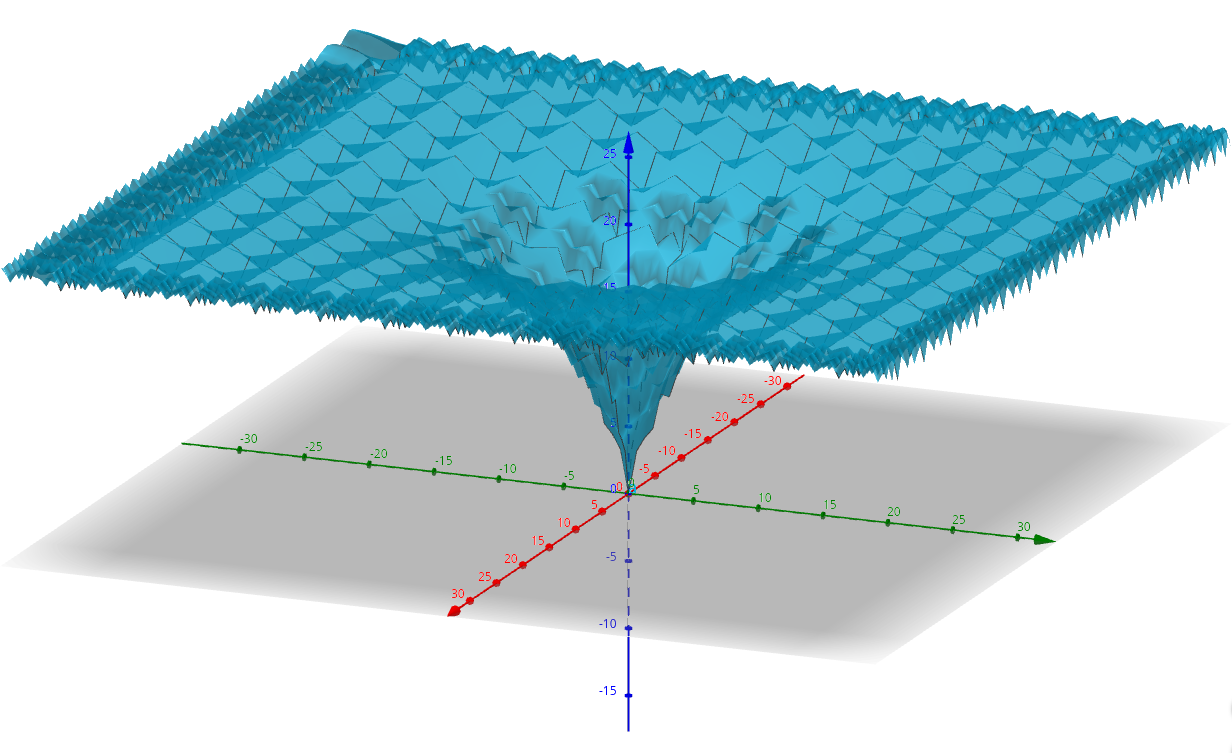
\includegraphics[width=\textwidth]{funcion_3D.png}
\end{figure}

\FloatBarrier

Por lo que, por simple inspección, se esperaría que el mínimo fuera aproximadamente (0, 0).

\section{Implementación del algoritmo}

Antes de implementar el algoritmo genético, se deben definir los siguientes puntos:

\begin{enumerate}
    \item \textbf{Función de aptitud}

          Puesto que se busca minimizar el valor de la función, no se puede emplear
          la función directamente, sino que se debe multiplicar por $-1$. Sin embargo,
          usar $-f(x_1, x_2)$ produciría números negativos, lo que causaría problemas
          para la selección por ruleta, así que la función $-f(x_1, x_2) + 50$ resulta
          una función de evaluación adecuada.

    \item \textbf{Representación de las soluciones}

          Se tienen que representar números en el rango $[-32.768, 32.768]$, para
          lo cual se pueden emplear números en el rango $[-32768, 32768]$ y dividirlos
          entre $1000$. Más aún, como 32768 es exactamente $2^{15}$, cada variable se
          puede representar como un arreglo de 16 bits, y toda la solución como un
          arreglo de 32 bits.

    \item \textbf{Población inicial}

          Como se decidió representar cada solución como un arreglo de 32 bits, resulta
          sencillo crear una población inicial con un número $x$ de individuos aleatorios,
          donde los bits de cada individuo tengan un $50\percentsign$ de probabilidad de
          ser $1$ o $0$.

    \item \textbf{Criterio de paro}

          El criterio de paro que resultó conveniente para este proyecto fue el de
          detener la ejecución tras transcurrir $10,000$ iteraciones sin encontrar
          una mejor solución.
\end{enumerate}

Para la implementación del algoritmo, se decidió usar el lenguaje de programación
Rust. El cual resulta conveniente para esta tarea por diversas razonas,
la principal es que, como se trata de un lenguaje compilado de bajo nivel,
permite generar código eficiente, lo que resulta conveniente puesto que cada
ejecución requerirá de miles de iteraciones del algoritmo.

El código se puede encontrar al final de este documento.

\section{Análisis}

A continuación se presenta un análisis de los efectos que tienen diversas variables
en los resultados del algoritmo. Específicamente, se realizaron cientos de ejecuciones
variando uno por uno los valores de tamaño de la población, probabilidad de cruza, probabilidad
de mutación, función de cruza y función de selección, mientras que el resto de los
valores se fijaron como constantes.

\pagebreak

\figuras{variacion_tam_pop}{Resultados promedio al variar el tamaño de la población}

La figura \ref{fig:variacion_tam_pop} muestra los resultados de variar el tamaño
de la población entre 50 y 200. Las probabilidades de cruza y mutación se fijaron
en 0.25 y 0.01 respectivamente. Se empleó cruza en un punto y selección por torneo.
Cada punto en la gráfica representa el promedio de 100 ejecuciones del algoritmo
con los valores correspondientes.

La figura \ref{fig:variacion_tam_pop_1} muestra el promedio de la aptitud de la
población que se obtuvo al final de la ejecución (Después de $10,000$ iteraciones
sin mejora) y la figura \ref{fig:variacion_tam_pop_2} muestra el promedio de la
aptitude del mejor individuo que se encontró durante la ejecución.

Como se puede observar, el tamaño de la población no parece tener un efecto
significativo en el resultado final del algoritmo.

La figura \ref{fig:variacion_tam_pop_3} muestra el promedio de la cantidad de
iteraciones que le llevó al algoritmo encontrar al mejor individuo. Esto quiere
decir que, como el algoritmo se detiene después de $10,000$ iteraciones sin encontrar
un mejor individuo, la cantidad de iteraciones que transcurren antes de encontrar
a dicho individuo se calcula restando $10,000$ al número total de iteraciones
transcurridas.

Esto nos muestra que el algoritmo requirió de significativamente menos iteraciones
para encontrar una buena solución cuando se contaban con poblaciones más grandes.
Sin embargo, como se puede ver en la figura \ref{fig:variacion_tam_pop_4}, esta
ganancia es contrarrestada por el hecho de que las iteraciones con poblaciones
mayores consumen más tiempo.

Por esta razón es que se escogió 50 como tamaño de la población para ejecuciones
futuras, puesto que permite ahorrar tiempo de ejecución sin sacrificar la calidad
de los resultados finales.

A continuación se analizarán los efectos de variar la probabilidad de cruza.

\figuras{variacion_probabilidad_cruza_1}{Resultados promedio al variar la probabilidad de cruza}

\figuras{variacion_probabilidad_cruza_2}{Resultados promedio al variar la probabilidad de cruza (300 ejecuciones)}

La figura \ref{fig:variacion_probabilidad_cruza_1} se obtuvo de forma semejante
a la figura \ref{fig:variacion_tam_pop}, pero esta vez fijando la población en 50
y variando la probabilidad de cruza entre 0.1 y 0.25.

Al igual que en el caso anterior, variar la probabilidad de cruza entre estos valores
no parece tener ningún efecto en los resultados finales (Figuras
\ref{fig:variacion_probabilidad_cruza_1_1} y \ref{fig:variacion_probabilidad_cruza_1_2}).
Sin embargo, a diferencia del caso anterior, no parece tener ningún efecto en
la cantidad de iteraciones requeridas. Para confirmar esta hipótesis, se realizaron
las ejecuciones que se ven en la figura \ref{fig:variacion_probabilidad_cruza_2},
las cuales se llevaron acabo con los mismos parámetros que las de la figura
\ref{fig:variacion_probabilidad_cruza_1}, pero promediando 300 ejecuciones con cada
probabilidad de cruza, en lugar de 100.

En efecto, los resultados de este nuevo conjunto de ejecuciones son muy semejantes
a los anteriormente producidos.

Curiosamente, se percibe una ligera mejora en tiempo de ejecución cuando se tiene
menor probabilidad de cruza (figuras \ref{fig:variacion_probabilidad_cruza_2_4} y
\ref{fig:variacion_probabilidad_cruza_1_4}), probablemente debido al tiempo que
se ahorra al aplicar el algoritmo de cruza menos veces, puesto que en promedio
se selecciona a menos individuos para ser cruzados. Por esta razón se decidió
usar una probabilidad de cruza de 0.1 para ejecuciones futuras.

Ahora veremos los resultados de variar la probabilidad de mutación.

\figuras{variacion_probabilidad_mutacion}{Resultados promedio al variar la probabilidad de mutación}

Los datos de la figura \ref{fig:variacion_probabilidad_mutacion} se obtuvieron
de forma semejante a los de las figuras \ref{fig:variacion_probabilidad_cruza_1} y
\ref{fig:variacion_probabilidad_cruza_2} pero ahora fijando la probabilidad de cruza
en $0.1$ y variando la probabilidad de mutación entre $0.01$ y $0.05$. Se realizaron 100
ejecuciones con cada probabilidad de mutación.

Con un simple vistazo a la figura \ref{fig:variacion_probabilidad_mutacion_1}
resulta claro que mientras mayor sea la probabilidad de mutación, menor será la aptitud
promedio de la población final. Esto tiene sentido, puesto que al ser completamente
aleatorias, las mutaciones evitan que la población se estabilice tanto en valores
de aptitud muy altos como muy bajos.

Sin embargo, como muestra la figura \ref{fig:variacion_probabilidad_mutacion_2},
este decremento en aptitud promedio no necesariamente se traduce en peores soluciones
finales. Se puede conjeturar que, para probabilidades de mutación entre $0.01$ y $0.04$,
se sigue teniendo un balance aceptable entre exploración y explotación por lo que
se siguen obteniendo soluciones razonablemente buenas, sin embargo, para valores
mayores a $0.04$ se empieza a contar con demasiada exploración, teniendo como
resultado el hallazgo de peores soluciones.

Las figuras \ref{fig:variacion_probabilidad_mutacion_3} y
\ref{fig:variacion_probabilidad_mutacion_4} muestran que la cantidad de iteraciones
y el tiempo de ejecución aumentan exponencialmente a medida que aumenta la
probabilidad de mutación, puesto que mientras más aumenta esta probabilidad, más
se acerca el algoritmo a ser una simple búsqueda aleatoria por ensayo y error.

La probabilidad de mutación que resulta más conveniente es entonces $0.01$;

Lo siguiente será comparar las funciones de cruza y de selección.

\figuras{variacion_funcion_seleccion}{Resultados promedio de selección por ruleta y por torneo}

\figuras{variacion_funcion_cruza}{Resultados promedio de cruza por un punto y dos puntos}

Las datos para las figuras \ref{fig:variacion_funcion_seleccion} y
\ref{fig:variacion_funcion_cruza} fueron obtenidos con una población de tamaño 50
y probabilidades de cruza y mutación de $0.1$ y $0.01$ respectivamente. Se
promediaron $500$ ejecuciones para cada función de selección y $1500$ para cada
función de cruza.

Como es de esperar, la selección por ruleta produce resultados mucho peores que
la selección por torneo en términos de aptitud de la población final (Figura
\ref{fig:variacion_funcion_seleccion_1}), cantidad de iteraciones (Figura
\ref{fig:variacion_funcion_seleccion_3}) y, como consecuencia, tiempo de ejecución
(Figura \ref{fig:variacion_funcion_seleccion_4}). Incluso la aptitud promedio
de la solución final es ligeramente peor con selección por ruleta (Figura
\ref{fig:variacion_funcion_seleccion_2}).

Por otra parte, no hay ninguna diferencia significativa entre el uso de cruza en
un punto comparado con la cruza en dos puntos.

\pagebreak

\section{Resultado final}

Habiendo realizado el análisis anterior, se puede entonces realizar múltiples
ejecuciones del programa en búsqueda del mínimo de la función. Para ello se
utilizará una población de 50 individuos, probabilidades de cruza y mutación de
$0.1$ y $0.01$ respectivamente, selección por torneo y cruza en un punto.

La siguiente tabla muestra los resultados de 20 ejecuciones del programa, ordenadas
de mayor a menor según la aptitud del mejor individuo. Para cada ejecución se
registró la aptitud promedio de la población final, la aptitud del mejor individuo,
la cantidad de iteraciones que llevó encontrar dicho individuo, el tiempo que llevó
la ejecución y el valor del mejor individuo.

Como se puede ver, los mejores valores encontrados por el algoritmo fueron
$x_1 = 0$ y $x_2 = 0$. Evaluando en la función, obtenemos que $f(0, 0) = 0$.

\pgfplotstabletypeset[
    columns/1/.style={column name={Aptitud población}},
    columns/2/.style={column name={Aptitud mejor individuo}},
    columns/3/.style={column name={Iteraciones}},
    columns/4/.style={column name={Tiempo (S)}},
    columns/5/.style={column name={Mejor individuo}},
    columns={1,2,3,4,5},
    header=false,
    string type,
    before row=\hline,
    every last row/.style={after row=\hline},
    column type/.add={|}{},
    every last column/.style={column type/.add={}{|}},
    text indicator="
]{../datos_ejecuciones/20_ejecuciones.txt}%

\pagebreak

\section{Código}

\inputminted[
    linenos,
    breaklines,
    bgcolor=LightGray,
    label=lib.rs,
    labelposition=all,
    frame=topline
]
{rust}{../src/lib.rs}


\inputminted[
    linenos,
    breaklines,
    bgcolor=LightGray,
    label=main.rs,
    labelposition=all,
    frame=topline
]
{rust}{../src/main.rs}

\end{document}